\documentclass[1p]{elsarticle_modified}
%\bibliographystyle{elsarticle-num}

%\usepackage[colorlinks]{hyperref}
%\usepackage{abbrmath_seonhwa} %\Abb, \Ascr, \Acal ,\Abf, \Afrak
\usepackage{amsfonts}
\usepackage{amssymb}
\usepackage{amsmath}
\usepackage{amsthm}
\usepackage{scalefnt}
\usepackage{amsbsy}
\usepackage{kotex}
\usepackage{caption}
\usepackage{subfig}
\usepackage{color}
\usepackage{graphicx}
\usepackage{xcolor} %% white, black, red, green, blue, cyan, magenta, yellow
\usepackage{float}
\usepackage{setspace}
\usepackage{hyperref}

\usepackage{tikz}
\usetikzlibrary{arrows}

\usepackage{multirow}
\usepackage{array} % fixed length table
\usepackage{hhline}

%%%%%%%%%%%%%%%%%%%%%
\makeatletter
\renewcommand*\env@matrix[1][\arraystretch]{%
	\edef\arraystretch{#1}%
	\hskip -\arraycolsep
	\let\@ifnextchar\new@ifnextchar
	\array{*\c@MaxMatrixCols c}}
\makeatother %https://tex.stackexchange.com/questions/14071/how-can-i-increase-the-line-spacing-in-a-matrix
%%%%%%%%%%%%%%%

\usepackage[normalem]{ulem}

\newcommand{\msout}[1]{\ifmmode\text{\sout{\ensuremath{#1}}}\else\sout{#1}\fi}
%SOURCE: \msout is \stkout macro in https://tex.stackexchange.com/questions/20609/strikeout-in-math-mode

\newcommand{\cancel}[1]{
	\ifmmode
	{\color{red}\msout{#1}}
	\else
	{\color{red}\sout{#1}}
	\fi
}

\newcommand{\add}[1]{
	{\color{blue}\uwave{#1}}
}

\newcommand{\replace}[2]{
	\ifmmode
	{\color{red}\msout{#1}}{\color{blue}\uwave{#2}}
	\else
	{\color{red}\sout{#1}}{\color{blue}\uwave{#2}}
	\fi
}

\newcommand{\Sol}{\mathcal{S}} %segment
\newcommand{\D}{D} %diagram
\newcommand{\A}{\mathcal{A}} %arc


%%%%%%%%%%%%%%%%%%%%%%%%%%%%%5 test

\def\sl{\operatorname{\textup{SL}}(2,\Cbb)}
\def\psl{\operatorname{\textup{PSL}}(2,\Cbb)}
\def\quan{\mkern 1mu \triangleright \mkern 1mu}

\theoremstyle{definition}
\newtheorem{thm}{Theorem}[section]
\newtheorem{prop}[thm]{Proposition}
\newtheorem{lem}[thm]{Lemma}
\newtheorem{ques}[thm]{Question}
\newtheorem{cor}[thm]{Corollary}
\newtheorem{defn}[thm]{Definition}
\newtheorem{exam}[thm]{Example}
\newtheorem{rmk}[thm]{Remark}
\newtheorem{alg}[thm]{Algorithm}

\newcommand{\I}{\sqrt{-1}}
\begin{document}

%\begin{frontmatter}
%
%\title{Boundary parabolic representations of knots up to 8 crossings}
%
%%% Group authors per affiliation:
%\author{Yunhi Cho} 
%\address{Department of Mathematics, University of Seoul, Seoul, Korea}
%\ead{yhcho@uos.ac.kr}
%
%
%\author{Seonhwa Kim} %\fnref{s_kim}}
%\address{Center for Geometry and Physics, Institute for Basic Science, Pohang, 37673, Korea}
%\ead{ryeona17@ibs.re.kr}
%
%\author{Hyuk Kim}
%\address{Department of Mathematical Sciences, Seoul National University, Seoul 08826, Korea}
%\ead{hyukkim@snu.ac.kr}
%
%\author{Seokbeom Yoon}
%\address{Department of Mathematical Sciences, Seoul National University, Seoul, 08826,  Korea}
%\ead{sbyoon15@snu.ac.kr}
%
%\begin{abstract}
%We find all boundary parabolic representation of knots up to 8 crossings.
%
%\end{abstract}
%\begin{keyword}
%    \MSC[2010] 57M25 
%\end{keyword}
%
%\end{frontmatter}

%\linenumbers
%\tableofcontents
%
\newcommand\colored[1]{\textcolor{white}{\rule[-0.35ex]{0.8em}{1.4ex}}\kern-0.8em\color{red} #1}%
%\newcommand\colored[1]{\textcolor{white}{ #1}\kern-2.17ex	\textcolor{white}{ #1}\kern-1.81ex	\textcolor{white}{ #1}\kern-2.15ex\color{red}#1	}

{\Large $\underline{11a_{298}~(K11a_{298})}$}

\setlength{\tabcolsep}{10pt}
\renewcommand{\arraystretch}{1.6}
\vspace{1cm}\begin{tabular}{m{100pt}>{\centering\arraybackslash}m{274pt}}
\multirow{5}{120pt}{
	\centering
	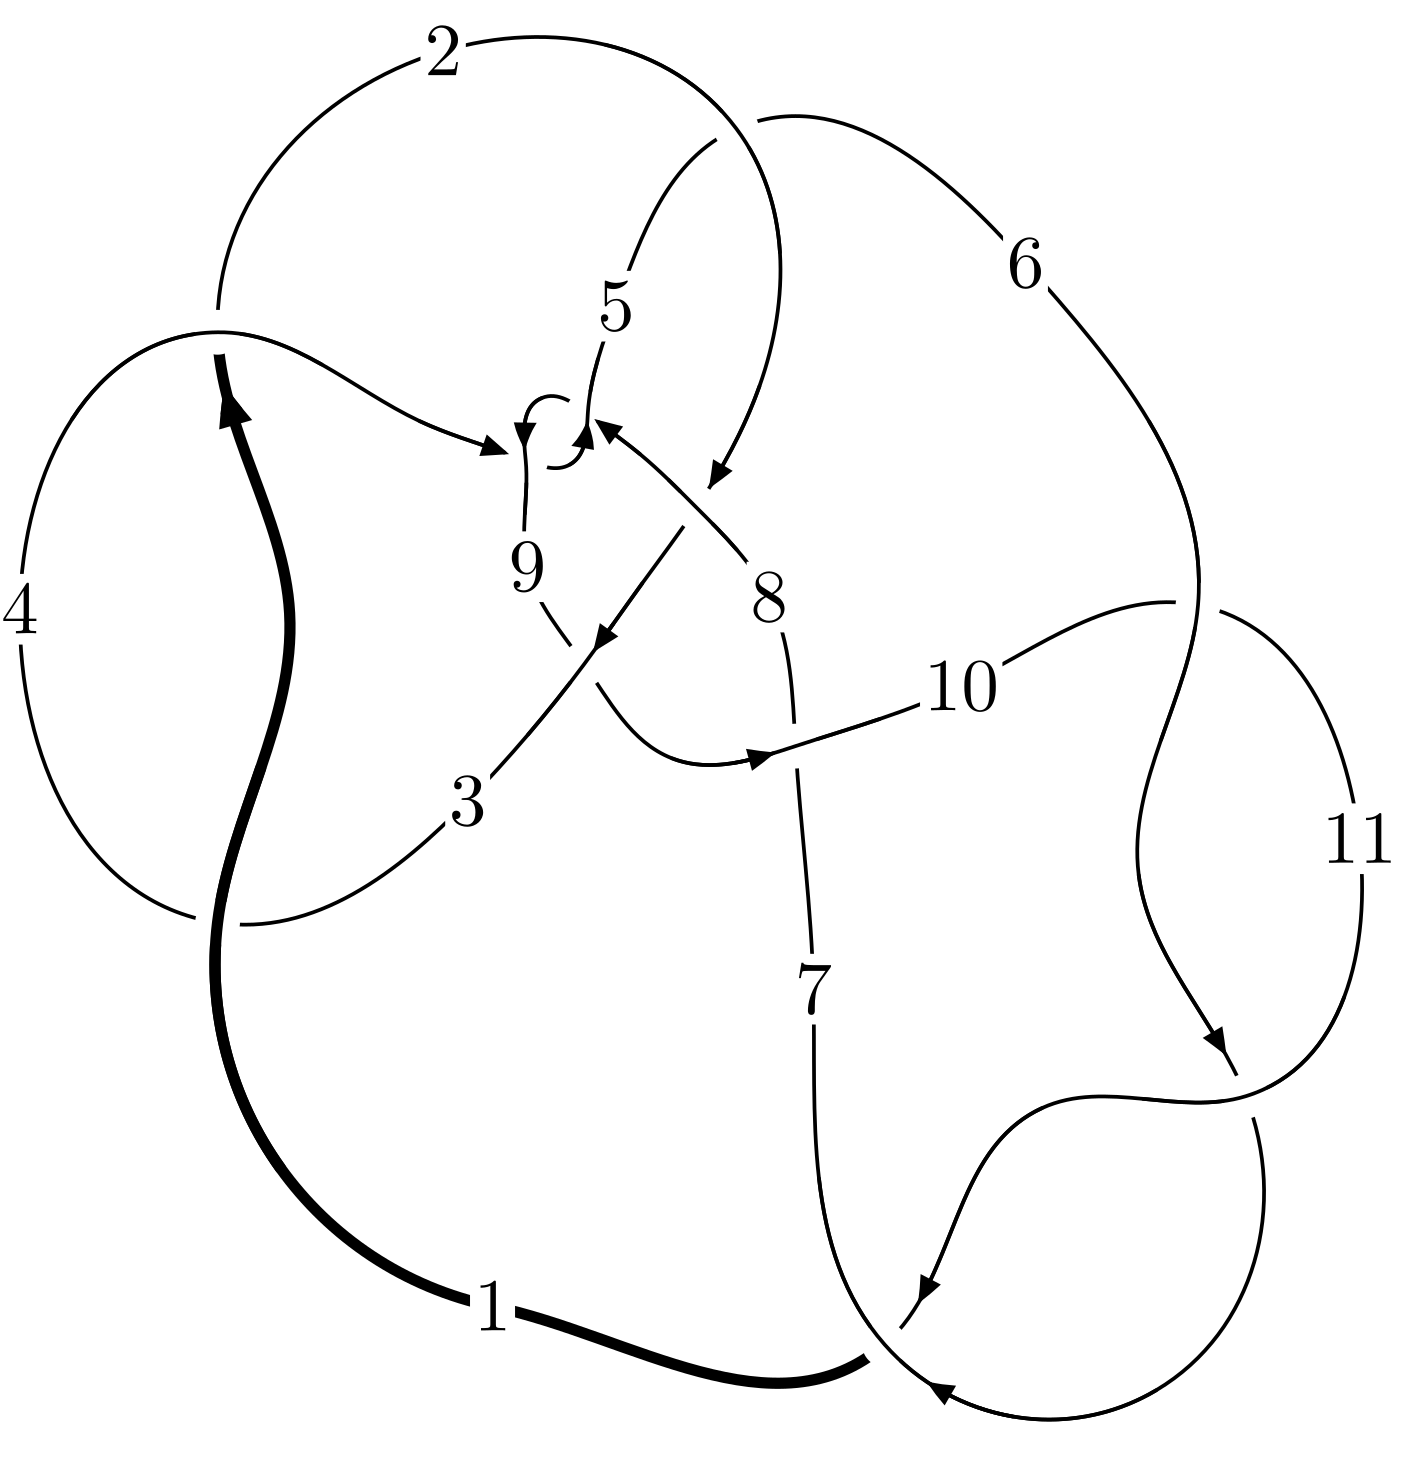
\includegraphics[width=112pt]{../../../GIT/diagram.site/Diagrams/png/547_11a_298.png}\\
\ \ \ A knot diagram\footnotemark}&
\allowdisplaybreaks
\textbf{Linearized knot diagam} \\
\cline{2-2}
 &
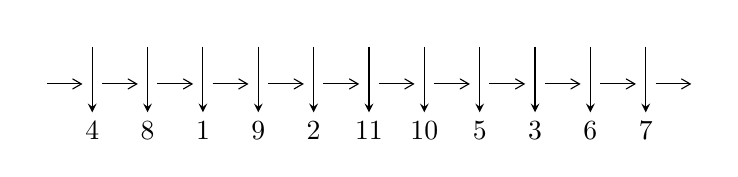
\begin{tikzpicture}[x=20pt, y=17pt]
	% nodes
	\node (C0) at (0, 0) {};
	\node (C1) at (1, 0) {};
	\node (C1U) at (1, +1) {};
	\node (C1D) at (1, -1) {4};

	\node (C2) at (2, 0) {};
	\node (C2U) at (2, +1) {};
	\node (C2D) at (2, -1) {8};

	\node (C3) at (3, 0) {};
	\node (C3U) at (3, +1) {};
	\node (C3D) at (3, -1) {1};

	\node (C4) at (4, 0) {};
	\node (C4U) at (4, +1) {};
	\node (C4D) at (4, -1) {9};

	\node (C5) at (5, 0) {};
	\node (C5U) at (5, +1) {};
	\node (C5D) at (5, -1) {2};

	\node (C6) at (6, 0) {};
	\node (C6U) at (6, +1) {};
	\node (C6D) at (6, -1) {11};

	\node (C7) at (7, 0) {};
	\node (C7U) at (7, +1) {};
	\node (C7D) at (7, -1) {10};

	\node (C8) at (8, 0) {};
	\node (C8U) at (8, +1) {};
	\node (C8D) at (8, -1) {5};

	\node (C9) at (9, 0) {};
	\node (C9U) at (9, +1) {};
	\node (C9D) at (9, -1) {3};

	\node (C10) at (10, 0) {};
	\node (C10U) at (10, +1) {};
	\node (C10D) at (10, -1) {6};

	\node (C11) at (11, 0) {};
	\node (C11U) at (11, +1) {};
	\node (C11D) at (11, -1) {7};
	\node (C12) at (12, 0) {};

	% arrows
	\draw[->,>={angle 60}]
	(C0) edge (C1) (C1) edge (C2) (C2) edge (C3) (C3) edge (C4) (C4) edge (C5) (C5) edge (C6) (C6) edge (C7) (C7) edge (C8) (C8) edge (C9) (C9) edge (C10) (C10) edge (C11) (C11) edge (C12) ;	\draw[->,>=stealth]
	(C1U) edge (C1D) (C2U) edge (C2D) (C3U) edge (C3D) (C4U) edge (C4D) (C5U) edge (C5D) (C6U) edge (C6D) (C7U) edge (C7D) (C8U) edge (C8D) (C9U) edge (C9D) (C10U) edge (C10D) (C11U) edge (C11D) ;
	\end{tikzpicture} \\
\hhline{~~} \\& 
\textbf{Solving Sequence} \\ \cline{2-2} 
 &
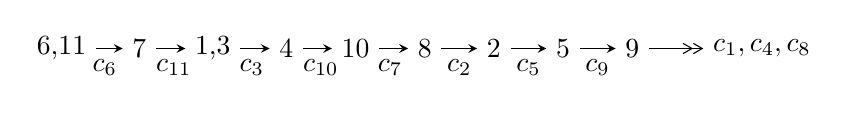
\begin{tikzpicture}[x=25pt, y=7pt]
	% node
	\node (A0) at (-1/8, 0) {6,11};
	\node (A1) at (1, 0) {7};
	\node (A2) at (33/16, 0) {1,3};
	\node (A3) at (25/8, 0) {4};
	\node (A4) at (33/8, 0) {10};
	\node (A5) at (41/8, 0) {8};
	\node (A6) at (49/8, 0) {2};
	\node (A7) at (57/8, 0) {5};
	\node (A8) at (65/8, 0) {9};
	\node (C1) at (1/2, -1) {$c_{6}$};
	\node (C2) at (3/2, -1) {$c_{11}$};
	\node (C3) at (21/8, -1) {$c_{3}$};
	\node (C4) at (29/8, -1) {$c_{10}$};
	\node (C5) at (37/8, -1) {$c_{7}$};
	\node (C6) at (45/8, -1) {$c_{2}$};
	\node (C7) at (53/8, -1) {$c_{5}$};
	\node (C8) at (61/8, -1) {$c_{9}$};
	\node (A9) at (10, 0) {$c_{1},c_{4},c_{8}$};

	% edge
	\draw[->,>=stealth]	
	(A0) edge (A1) (A1) edge (A2) (A2) edge (A3) (A3) edge (A4) (A4) edge (A5) (A5) edge (A6) (A6) edge (A7) (A7) edge (A8) ;
	\draw[->>,>={angle 60}]	
	(A8) edge (A9);
\end{tikzpicture} \\ 

\end{tabular} \\

\footnotetext{
The image of knot diagram is generated by the software ``\textbf{Draw programme}" developed by Andrew Bartholomew(\url{http://www.layer8.co.uk/maths/draw/index.htm\#Running-draw}), where we modified some parts for our purpose(\url{https://github.com/CATsTAILs/LinksPainter}).
}\phantom \\ \newline 
\centering \textbf{Ideals for irreducible components\footnotemark of $X_{\text{par}}$} 
 
\begin{align*}
I^u_{1}&=\langle 
9.88613\times10^{36} u^{66}-3.08299\times10^{36} u^{65}+\cdots+2.08415\times10^{37} b+1.52499\times10^{37},\\
\phantom{I^u_{1}}&\phantom{= \langle  }-1.79254\times10^{37} u^{66}-3.42174\times10^{37} u^{65}+\cdots+2.08415\times10^{37} a-3.54411\times10^{37},\;u^{67}+2 u^{66}+\cdots+2 u+1\rangle \\
I^u_{2}&=\langle 
5 b+u+3,\;5 a+2 u+6,\;u^2+u-1\rangle \\
\\
\end{align*}
\raggedright * 2 irreducible components of $\dim_{\mathbb{C}}=0$, with total 69 representations.\\
\footnotetext{All coefficients of polynomials are rational numbers. But the coefficients are sometimes approximated in decimal forms when there is not enough margin.}
\newpage
\renewcommand{\arraystretch}{1}
\centering \section*{I. $I^u_{1}= \langle 9.89\times10^{36} u^{66}-3.08\times10^{36} u^{65}+\cdots+2.08\times10^{37} b+1.52\times10^{37},\;-1.79\times10^{37} u^{66}-3.42\times10^{37} u^{65}+\cdots+2.08\times10^{37} a-3.54\times10^{37},\;u^{67}+2 u^{66}+\cdots+2 u+1 \rangle$}
\flushleft \textbf{(i) Arc colorings}\\
\begin{tabular}{m{7pt} m{180pt} m{7pt} m{180pt} }
\flushright $a_{6}=$&$\begin{pmatrix}1\\0\end{pmatrix}$ \\
\flushright $a_{11}=$&$\begin{pmatrix}0\\u\end{pmatrix}$ \\
\flushright $a_{7}=$&$\begin{pmatrix}1\\u^2\end{pmatrix}$ \\
\flushright $a_{1}=$&$\begin{pmatrix}- u\\- u^3+u\end{pmatrix}$ \\
\flushright $a_{3}=$&$\begin{pmatrix}0.860082 u^{66}+1.64179 u^{65}+\cdots+1.94258 u+1.70050\\-0.474347 u^{66}+0.147925 u^{65}+\cdots-0.386242 u-0.731707\end{pmatrix}$ \\
\flushright $a_{4}=$&$\begin{pmatrix}1.48932 u^{66}+2.14476 u^{65}+\cdots+3.32469 u+2.19964\\-0.127700 u^{66}+0.342656 u^{65}+\cdots-0.886592 u-0.475343\end{pmatrix}$ \\
\flushright $a_{10}=$&$\begin{pmatrix}u\\u\end{pmatrix}$ \\
\flushright $a_{8}=$&$\begin{pmatrix}- u^4+u^2+1\\- u^4+2 u^2\end{pmatrix}$ \\
\flushright $a_{2}=$&$\begin{pmatrix}0.788597 u^{66}+1.72240 u^{65}+\cdots+3.47709 u+1.64125\\-0.360672 u^{66}+0.258719 u^{65}+\cdots-0.433561 u-0.659189\end{pmatrix}$ \\
\flushright $a_{5}=$&$\begin{pmatrix}1.04231 u^{66}+1.25813 u^{65}+\cdots+2.97728 u+1.55836\\0.579023 u^{66}+0.216659 u^{65}+\cdots+0.557709 u+0.726240\end{pmatrix}$ \\
\flushright $a_{9}=$&$\begin{pmatrix}-1.54293 u^{66}-2.24497 u^{65}+\cdots-2.88258 u-2.33342\\-1.53821 u^{66}-1.11120 u^{65}+\cdots+0.768914 u-0.642905\end{pmatrix}$\\ \flushright $a_{9}=$&$\begin{pmatrix}-1.54293 u^{66}-2.24497 u^{65}+\cdots-2.88258 u-2.33342\\-1.53821 u^{66}-1.11120 u^{65}+\cdots+0.768914 u-0.642905\end{pmatrix}$\\&\end{tabular}
\flushleft \textbf{(ii) Obstruction class $= -1$}\\~\\
\flushleft \textbf{(iii) Cusp Shapes $= -2.85040 u^{66}-2.35907 u^{65}+\cdots+11.1605 u-13.3066$}\\~\\
\newpage\renewcommand{\arraystretch}{1}
\flushleft \textbf{(iv) u-Polynomials at the component}\newline \\
\begin{tabular}{m{50pt}|m{274pt}}
Crossings & \hspace{64pt}u-Polynomials at each crossing \\
\hline $$\begin{aligned}c_{1},c_{3}\end{aligned}$$&$\begin{aligned}
&u^{67}-3 u^{66}+\cdots-11 u+25
\end{aligned}$\\
\hline $$\begin{aligned}c_{2}\end{aligned}$$&$\begin{aligned}
&u^{67}+u^{66}+\cdots+980 u+100
\end{aligned}$\\
\hline $$\begin{aligned}c_{4},c_{8}\end{aligned}$$&$\begin{aligned}
&u^{67}+2 u^{66}+\cdots+4 u+1
\end{aligned}$\\
\hline $$\begin{aligned}c_{5}\end{aligned}$$&$\begin{aligned}
&5(5 u^{67}-44 u^{66}+\cdots+396 u+27)
\end{aligned}$\\
\hline $$\begin{aligned}c_{6},c_{10},c_{11}\end{aligned}$$&$\begin{aligned}
&u^{67}+2 u^{66}+\cdots+2 u+1
\end{aligned}$\\
\hline $$\begin{aligned}c_{7}\end{aligned}$$&$\begin{aligned}
&u^{67}-6 u^{66}+\cdots-618 u+117
\end{aligned}$\\
\hline $$\begin{aligned}c_{9}\end{aligned}$$&$\begin{aligned}
&5(5 u^{67}+27 u^{66}+\cdots+819 u+81)
\end{aligned}$\\
\hline
\end{tabular}\\~\\
\newpage\renewcommand{\arraystretch}{1}
\flushleft \textbf{(v) Riley Polynomials at the component}\newline \\
\begin{tabular}{m{50pt}|m{274pt}}
Crossings & \hspace{64pt}Riley Polynomials at each crossing \\
\hline $$\begin{aligned}c_{1},c_{3}\end{aligned}$$&$\begin{aligned}
&y^{67}-39 y^{66}+\cdots+25671 y-625
\end{aligned}$\\
\hline $$\begin{aligned}c_{2}\end{aligned}$$&$\begin{aligned}
&y^{67}+15 y^{66}+\cdots+203000 y-10000
\end{aligned}$\\
\hline $$\begin{aligned}c_{4},c_{8}\end{aligned}$$&$\begin{aligned}
&y^{67}+36 y^{66}+\cdots+4 y-1
\end{aligned}$\\
\hline $$\begin{aligned}c_{5}\end{aligned}$$&$\begin{aligned}
&25(25 y^{67}+624 y^{66}+\cdots+130896 y-729)
\end{aligned}$\\
\hline $$\begin{aligned}c_{6},c_{10},c_{11}\end{aligned}$$&$\begin{aligned}
&y^{67}-60 y^{66}+\cdots+4 y-1
\end{aligned}$\\
\hline $$\begin{aligned}c_{7}\end{aligned}$$&$\begin{aligned}
&y^{67}+4 y^{66}+\cdots+137160 y-13689
\end{aligned}$\\
\hline $$\begin{aligned}c_{9}\end{aligned}$$&$\begin{aligned}
&25(25 y^{67}-79 y^{66}+\cdots-46413 y-6561)
\end{aligned}$\\
\hline
\end{tabular}\\~\\
\newpage\flushleft \textbf{(vi) Complex Volumes and Cusp Shapes}
$$\begin{array}{c|c|c}  
\text{Solutions to }I^u_{1}& \I (\text{vol} + \sqrt{-1}CS) & \text{Cusp shape}\\
 \hline 
\begin{aligned}
u &= \phantom{-}0.971049 + 0.208920 I \\
a &= -0.32714 + 1.78126 I \\
b &= -0.115970 + 0.555157 I\end{aligned}
 & \phantom{-}3.33579 + 2.19465 I & -7.86655 + 0. I\phantom{ +0.000000I} \\ \hline\begin{aligned}
u &= \phantom{-}0.971049 - 0.208920 I \\
a &= -0.32714 - 1.78126 I \\
b &= -0.115970 - 0.555157 I\end{aligned}
 & \phantom{-}3.33579 - 2.19465 I & -7.86655 + 0. I\phantom{ +0.000000I} \\ \hline\begin{aligned}
u &= \phantom{-}0.828642 + 0.456356 I \\
a &= \phantom{-}1.29398 - 1.09741 I \\
b &= \phantom{-}0.975419 + 0.388481 I\end{aligned}
 & \phantom{-}0.61572 + 7.81558 I & -11.00000 - 4.31786 I \\ \hline\begin{aligned}
u &= \phantom{-}0.828642 - 0.456356 I \\
a &= \phantom{-}1.29398 + 1.09741 I \\
b &= \phantom{-}0.975419 - 0.388481 I\end{aligned}
 & \phantom{-}0.61572 - 7.81558 I & -11.00000 + 4.31786 I \\ \hline\begin{aligned}
u &= -0.785572 + 0.521754 I \\
a &= -0.876770 - 0.752417 I \\
b &= -0.765978 + 0.288301 I\end{aligned}
 & -2.70603 - 1.76569 I & -13.31586 + 3.73920 I \\ \hline\begin{aligned}
u &= -0.785572 - 0.521754 I \\
a &= -0.876770 + 0.752417 I \\
b &= -0.765978 - 0.288301 I\end{aligned}
 & -2.70603 + 1.76569 I & -13.31586 - 3.73920 I \\ \hline\begin{aligned}
u &= \phantom{-}1.025940 + 0.403064 I \\
a &= \phantom{-}0.638976 + 1.070100 I \\
b &= \phantom{-}0.056372 + 0.523175 I\end{aligned}
 & \phantom{-}1.33655 - 6.86297 I & \phantom{-0.000000 } 0 \\ \hline\begin{aligned}
u &= \phantom{-}1.025940 - 0.403064 I \\
a &= \phantom{-}0.638976 - 1.070100 I \\
b &= \phantom{-}0.056372 - 0.523175 I\end{aligned}
 & \phantom{-}1.33655 + 6.86297 I & \phantom{-0.000000 } 0 \\ \hline\begin{aligned}
u &= -0.298287 + 0.796077 I \\
a &= \phantom{-}0.133666 - 0.260488 I \\
b &= -1.30707 - 0.75572 I\end{aligned}
 & -1.12210 + 6.34169 I & -11.92397 - 6.79037 I \\ \hline\begin{aligned}
u &= -0.298287 - 0.796077 I \\
a &= \phantom{-}0.133666 + 0.260488 I \\
b &= -1.30707 + 0.75572 I\end{aligned}
 & -1.12210 - 6.34169 I & -11.92397 + 6.79037 I\\
 \hline 
 \end{array}$$\newpage$$\begin{array}{c|c|c}  
\text{Solutions to }I^u_{1}& \I (\text{vol} + \sqrt{-1}CS) & \text{Cusp shape}\\
 \hline 
\begin{aligned}
u &= \phantom{-}0.272187 + 0.791950 I \\
a &= -0.230884 - 0.195053 I \\
b &= \phantom{-}1.67052 - 0.99999 I\end{aligned}
 & \phantom{-}2.41609 - 12.25380 I & -8.96204 + 8.44386 I \\ \hline\begin{aligned}
u &= \phantom{-}0.272187 - 0.791950 I \\
a &= -0.230884 + 0.195053 I \\
b &= \phantom{-}1.67052 + 0.99999 I\end{aligned}
 & \phantom{-}2.41609 + 12.25380 I & -8.96204 - 8.44386 I \\ \hline\begin{aligned}
u &= -1.133230 + 0.269613 I \\
a &= \phantom{-}0.275844 + 0.909490 I \\
b &= \phantom{-}0.184881 + 0.303565 I\end{aligned}
 & -1.02190 + 1.39824 I & \phantom{-0.000000 } 0 \\ \hline\begin{aligned}
u &= -1.133230 - 0.269613 I \\
a &= \phantom{-}0.275844 - 0.909490 I \\
b &= \phantom{-}0.184881 - 0.303565 I\end{aligned}
 & -1.02190 - 1.39824 I & \phantom{-0.000000 } 0 \\ \hline\begin{aligned}
u &= \phantom{-}0.140214 + 0.819901 I \\
a &= \phantom{-}0.116857 - 0.337825 I \\
b &= -0.481890 - 0.479676 I\end{aligned}
 & \phantom{-}4.07626 + 2.45751 I & -5.53723 - 4.39874 I \\ \hline\begin{aligned}
u &= \phantom{-}0.140214 - 0.819901 I \\
a &= \phantom{-}0.116857 + 0.337825 I \\
b &= -0.481890 + 0.479676 I\end{aligned}
 & \phantom{-}4.07626 - 2.45751 I & -5.53723 + 4.39874 I \\ \hline\begin{aligned}
u &= \phantom{-}0.311992 + 0.700971 I \\
a &= -0.145782 - 0.519209 I \\
b &= \phantom{-}1.343450 + 0.093089 I\end{aligned}
 & \phantom{-}4.46866 - 1.41400 I & -4.95439 + 4.71232 I \\ \hline\begin{aligned}
u &= \phantom{-}0.311992 - 0.700971 I \\
a &= -0.145782 + 0.519209 I \\
b &= \phantom{-}1.343450 - 0.093089 I\end{aligned}
 & \phantom{-}4.46866 + 1.41400 I & -4.95439 - 4.71232 I \\ \hline\begin{aligned}
u &= \phantom{-}0.195241 + 0.725393 I \\
a &= \phantom{-}0.102706 - 0.534072 I \\
b &= -1.42665 + 0.06702 I\end{aligned}
 & \phantom{-}5.66368 - 5.86500 I & -5.37991 + 6.33692 I \\ \hline\begin{aligned}
u &= \phantom{-}0.195241 - 0.725393 I \\
a &= \phantom{-}0.102706 + 0.534072 I \\
b &= -1.42665 - 0.06702 I\end{aligned}
 & \phantom{-}5.66368 + 5.86500 I & -5.37991 - 6.33692 I\\
 \hline 
 \end{array}$$\newpage$$\begin{array}{c|c|c}  
\text{Solutions to }I^u_{1}& \I (\text{vol} + \sqrt{-1}CS) & \text{Cusp shape}\\
 \hline 
\begin{aligned}
u &= -1.271530 + 0.161748 I \\
a &= \phantom{-}2.41947 + 0.73704 I \\
b &= \phantom{-}2.14316 - 0.56893 I\end{aligned}
 & -2.00089 + 2.82137 I & \phantom{-0.000000 } 0 \\ \hline\begin{aligned}
u &= -1.271530 - 0.161748 I \\
a &= \phantom{-}2.41947 - 0.73704 I \\
b &= \phantom{-}2.14316 + 0.56893 I\end{aligned}
 & -2.00089 - 2.82137 I & \phantom{-0.000000 } 0 \\ \hline\begin{aligned}
u &= -0.141220 + 0.702053 I \\
a &= -0.075965 - 0.431787 I \\
b &= \phantom{-}0.902832 + 0.342246 I\end{aligned}
 & \phantom{-}1.93198 + 2.14020 I & -7.90136 - 3.81097 I \\ \hline\begin{aligned}
u &= -0.141220 - 0.702053 I \\
a &= -0.075965 + 0.431787 I \\
b &= \phantom{-}0.902832 - 0.342246 I\end{aligned}
 & \phantom{-}1.93198 - 2.14020 I & -7.90136 + 3.81097 I \\ \hline\begin{aligned}
u &= \phantom{-}0.657943 + 0.240545 I \\
a &= -0.13672 - 1.54848 I \\
b &= \phantom{-}0.683159 - 0.173182 I\end{aligned}
 & \phantom{-}3.10200 - 2.24588 I & -7.87626 + 2.77695 I \\ \hline\begin{aligned}
u &= \phantom{-}0.657943 - 0.240545 I \\
a &= -0.13672 + 1.54848 I \\
b &= \phantom{-}0.683159 + 0.173182 I\end{aligned}
 & \phantom{-}3.10200 + 2.24588 I & -7.87626 - 2.77695 I \\ \hline\begin{aligned}
u &= \phantom{-}1.314170 + 0.128201 I \\
a &= -1.10038 + 1.03976 I \\
b &= -1.66093 + 0.85544 I\end{aligned}
 & -5.00722 - 0.73302 I & \phantom{-0.000000 } 0 \\ \hline\begin{aligned}
u &= \phantom{-}1.314170 - 0.128201 I \\
a &= -1.10038 - 1.03976 I \\
b &= -1.66093 - 0.85544 I\end{aligned}
 & -5.00722 + 0.73302 I & \phantom{-0.000000 } 0 \\ \hline\begin{aligned}
u &= -1.320040 + 0.057043 I \\
a &= \phantom{-}1.36174 + 0.91804 I \\
b &= \phantom{-}1.39912 + 1.18725 I\end{aligned}
 & -2.47273 - 2.48121 I & \phantom{-0.000000 } 0 \\ \hline\begin{aligned}
u &= -1.320040 - 0.057043 I \\
a &= \phantom{-}1.36174 - 0.91804 I \\
b &= \phantom{-}1.39912 - 1.18725 I\end{aligned}
 & -2.47273 + 2.48121 I & \phantom{-0.000000 } 0\\
 \hline 
 \end{array}$$\newpage$$\begin{array}{c|c|c}  
\text{Solutions to }I^u_{1}& \I (\text{vol} + \sqrt{-1}CS) & \text{Cusp shape}\\
 \hline 
\begin{aligned}
u &= \phantom{-}1.322170 + 0.229367 I \\
a &= \phantom{-}0.14439 - 7.47115 I \\
b &= \phantom{-}3.94009 - 5.01080 I\end{aligned}
 & -2.87450 - 2.88828 I & \phantom{-0.000000 } 0 \\ \hline\begin{aligned}
u &= \phantom{-}1.322170 - 0.229367 I \\
a &= \phantom{-}0.14439 + 7.47115 I \\
b &= \phantom{-}3.94009 + 5.01080 I\end{aligned}
 & -2.87450 + 2.88828 I & \phantom{-0.000000 } 0 \\ \hline\begin{aligned}
u &= -1.319590 + 0.346942 I \\
a &= -0.476943 + 0.014476 I \\
b &= -0.666723 + 0.083983 I\end{aligned}
 & -0.49228 + 1.74583 I & \phantom{-0.000000 } 0 \\ \hline\begin{aligned}
u &= -1.319590 - 0.346942 I \\
a &= -0.476943 - 0.014476 I \\
b &= -0.666723 - 0.083983 I\end{aligned}
 & -0.49228 - 1.74583 I & \phantom{-0.000000 } 0 \\ \hline\begin{aligned}
u &= -0.219881 + 0.595702 I \\
a &= \phantom{-}0.441318 + 0.005243 I \\
b &= \phantom{-}1.21996 + 0.96570 I\end{aligned}
 & \phantom{-}0.06257 + 4.19245 I & -10.29586 - 9.03236 I \\ \hline\begin{aligned}
u &= -0.219881 - 0.595702 I \\
a &= \phantom{-}0.441318 - 0.005243 I \\
b &= \phantom{-}1.21996 - 0.96570 I\end{aligned}
 & \phantom{-}0.06257 - 4.19245 I & -10.29586 + 9.03236 I \\ \hline\begin{aligned}
u &= \phantom{-}1.363670 + 0.157603 I \\
a &= -0.646817 - 0.030339 I \\
b &= -1.52794 + 0.21614 I\end{aligned}
 & -6.14223 - 0.20744 I & \phantom{-0.000000 } 0 \\ \hline\begin{aligned}
u &= \phantom{-}1.363670 - 0.157603 I \\
a &= -0.646817 + 0.030339 I \\
b &= -1.52794 - 0.21614 I\end{aligned}
 & -6.14223 + 0.20744 I & \phantom{-0.000000 } 0 \\ \hline\begin{aligned}
u &= -1.367670 + 0.191097 I \\
a &= -0.180450 - 1.153580 I \\
b &= \phantom{-}0.375829 - 0.704752 I\end{aligned}
 & -6.71014 + 3.51832 I & \phantom{-0.000000 } 0 \\ \hline\begin{aligned}
u &= -1.367670 - 0.191097 I \\
a &= -0.180450 + 1.153580 I \\
b &= \phantom{-}0.375829 + 0.704752 I\end{aligned}
 & -6.71014 - 3.51832 I & \phantom{-0.000000 } 0\\
 \hline 
 \end{array}$$\newpage$$\begin{array}{c|c|c}  
\text{Solutions to }I^u_{1}& \I (\text{vol} + \sqrt{-1}CS) & \text{Cusp shape}\\
 \hline 
\begin{aligned}
u &= \phantom{-}1.353030 + 0.281550 I \\
a &= \phantom{-}0.61601 - 1.37793 I \\
b &= \phantom{-}1.36173 - 1.14425 I\end{aligned}
 & -2.79764 - 5.70186 I & \phantom{-0.000000 } 0 \\ \hline\begin{aligned}
u &= \phantom{-}1.353030 - 0.281550 I \\
a &= \phantom{-}0.61601 + 1.37793 I \\
b &= \phantom{-}1.36173 + 1.14425 I\end{aligned}
 & -2.79764 + 5.70186 I & \phantom{-0.000000 } 0 \\ \hline\begin{aligned}
u &= -1.366210 + 0.216084 I \\
a &= -0.61315 - 2.12558 I \\
b &= -0.72885 - 1.51198 I\end{aligned}
 & -6.38128 + 3.82220 I & \phantom{-0.000000 } 0 \\ \hline\begin{aligned}
u &= -1.366210 - 0.216084 I \\
a &= -0.61315 + 2.12558 I \\
b &= -0.72885 + 1.51198 I\end{aligned}
 & -6.38128 - 3.82220 I & \phantom{-0.000000 } 0 \\ \hline\begin{aligned}
u &= -0.078148 + 0.604951 I \\
a &= -1.51809 - 0.93623 I \\
b &= \phantom{-}2.07351 + 2.80457 I\end{aligned}
 & \phantom{-}1.52367 - 0.14015 I & -14.2937 - 4.2199 I \\ \hline\begin{aligned}
u &= -0.078148 - 0.604951 I \\
a &= -1.51809 + 0.93623 I \\
b &= \phantom{-}2.07351 - 2.80457 I\end{aligned}
 & \phantom{-}1.52367 + 0.14015 I & -14.2937 + 4.2199 I \\ \hline\begin{aligned}
u &= \phantom{-}1.376960 + 0.239051 I \\
a &= \phantom{-}0.56095 - 2.53625 I \\
b &= \phantom{-}1.18970 - 2.28032 I\end{aligned}
 & -5.00444 - 7.26595 I & \phantom{-0.000000 } 0 \\ \hline\begin{aligned}
u &= \phantom{-}1.376960 - 0.239051 I \\
a &= \phantom{-}0.56095 + 2.53625 I \\
b &= \phantom{-}1.18970 + 2.28032 I\end{aligned}
 & -5.00444 + 7.26595 I & \phantom{-0.000000 } 0 \\ \hline\begin{aligned}
u &= -1.374450 + 0.292982 I \\
a &= -1.41785 - 1.33123 I \\
b &= -2.16228 - 0.85840 I\end{aligned}
 & \phantom{-}0.68934 + 9.55585 I & \phantom{-0.000000 } 0 \\ \hline\begin{aligned}
u &= -1.374450 - 0.292982 I \\
a &= -1.41785 + 1.33123 I \\
b &= -2.16228 + 0.85840 I\end{aligned}
 & \phantom{-}0.68934 - 9.55585 I & \phantom{-0.000000 } 0\\
 \hline 
 \end{array}$$\newpage$$\begin{array}{c|c|c}  
\text{Solutions to }I^u_{1}& \I (\text{vol} + \sqrt{-1}CS) & \text{Cusp shape}\\
 \hline 
\begin{aligned}
u &= -1.41838 + 0.31994 I \\
a &= \phantom{-}0.78576 + 2.39619 I \\
b &= \phantom{-}1.88722 + 1.70135 I\end{aligned}
 & -2.9681 + 16.2798 I & \phantom{-0.000000 } 0 \\ \hline\begin{aligned}
u &= -1.41838 - 0.31994 I \\
a &= \phantom{-}0.78576 - 2.39619 I \\
b &= \phantom{-}1.88722 - 1.70135 I\end{aligned}
 & -2.9681 - 16.2798 I & \phantom{-0.000000 } 0 \\ \hline\begin{aligned}
u &= \phantom{-}0.178834 + 0.510609 I \\
a &= -0.270334 + 1.049170 I \\
b &= -1.098170 + 0.533111 I\end{aligned}
 & -1.45952 - 1.07936 I & -12.77452 + 1.30331 I \\ \hline\begin{aligned}
u &= \phantom{-}0.178834 - 0.510609 I \\
a &= -0.270334 - 1.049170 I \\
b &= -1.098170 - 0.533111 I\end{aligned}
 & -1.45952 + 1.07936 I & -12.77452 - 1.30331 I \\ \hline\begin{aligned}
u &= \phantom{-}1.42924 + 0.31936 I \\
a &= -0.63124 + 1.94989 I \\
b &= -1.46734 + 1.38386 I\end{aligned}
 & -6.62942 - 10.38300 I & \phantom{-0.000000 } 0 \\ \hline\begin{aligned}
u &= \phantom{-}1.42924 - 0.31936 I \\
a &= -0.63124 - 1.94989 I \\
b &= -1.46734 - 1.38386 I\end{aligned}
 & -6.62942 + 10.38300 I & \phantom{-0.000000 } 0 \\ \hline\begin{aligned}
u &= -1.44421 + 0.28194 I \\
a &= \phantom{-}1.11075 + 1.15807 I \\
b &= \phantom{-}1.42474 + 0.38588 I\end{aligned}
 & -1.18945 + 5.01515 I & \phantom{-0.000000 } 0 \\ \hline\begin{aligned}
u &= -1.44421 - 0.28194 I \\
a &= \phantom{-}1.11075 - 1.15807 I \\
b &= \phantom{-}1.42474 - 0.38588 I\end{aligned}
 & -1.18945 - 5.01515 I & \phantom{-0.000000 } 0 \\ \hline\begin{aligned}
u &= -1.49701 + 0.03536 I \\
a &= \phantom{-}0.488640 - 0.267244 I \\
b &= -0.258686 - 0.678873 I\end{aligned}
 & -7.03449 - 6.70275 I & \phantom{-0.000000 } 0 \\ \hline\begin{aligned}
u &= -1.49701 - 0.03536 I \\
a &= \phantom{-}0.488640 + 0.267244 I \\
b &= -0.258686 + 0.678873 I\end{aligned}
 & -7.03449 + 6.70275 I & \phantom{-0.000000 } 0\\
 \hline 
 \end{array}$$\newpage$$\begin{array}{c|c|c}  
\text{Solutions to }I^u_{1}& \I (\text{vol} + \sqrt{-1}CS) & \text{Cusp shape}\\
 \hline 
\begin{aligned}
u &= \phantom{-}0.224112 + 0.424001 I \\
a &= -1.08363 + 1.63534 I \\
b &= -0.534595 + 0.408640 I\end{aligned}
 & -1.70121 - 1.12219 I & -12.55043 + 5.69637 I \\ \hline\begin{aligned}
u &= \phantom{-}0.224112 - 0.424001 I \\
a &= -1.08363 - 1.63534 I \\
b &= -0.534595 - 0.408640 I\end{aligned}
 & -1.70121 + 1.12219 I & -12.55043 - 5.69637 I \\ \hline\begin{aligned}
u &= \phantom{-}1.57577 + 0.03846 I \\
a &= -0.513955 - 0.003599 I \\
b &= -0.067086 - 0.129529 I\end{aligned}
 & -10.71130 + 0.03287 I & \phantom{-0.000000 } 0 \\ \hline\begin{aligned}
u &= \phantom{-}1.57577 - 0.03846 I \\
a &= -0.513955 + 0.003599 I \\
b &= -0.067086 + 0.129529 I\end{aligned}
 & -10.71130 - 0.03287 I & \phantom{-0.000000 } 0 \\ \hline\begin{aligned}
u &= -0.347952 + 0.238520 I \\
a &= \phantom{-}2.05729 + 1.92360 I \\
b &= -0.043214 + 0.259142 I\end{aligned}
 & -1.03011 - 1.52508 I & -14.1900 + 0.3808 I \\ \hline\begin{aligned}
u &= -0.347952 - 0.238520 I \\
a &= \phantom{-}2.05729 - 1.92360 I \\
b &= -0.043214 - 0.259142 I\end{aligned}
 & -1.03011 + 1.52508 I & -14.1900 - 0.3808 I \\ \hline\begin{aligned}
u &= -0.315598\phantom{ +0.000000I} \\
a &= \phantom{-}0.995497\phantom{ +0.000000I} \\
b &= -0.236639\phantom{ +0.000000I}\end{aligned}
 & -0.581693\phantom{ +0.000000I} & -17.2430\phantom{ +0.000000I}\\
 \hline 
 \end{array}$$\newpage\newpage\renewcommand{\arraystretch}{1}
\centering \section*{II. $I^u_{2}= \langle 5 b+u+3,\;5 a+2 u+6,\;u^2+u-1 \rangle$}
\flushleft \textbf{(i) Arc colorings}\\
\begin{tabular}{m{7pt} m{180pt} m{7pt} m{180pt} }
\flushright $a_{6}=$&$\begin{pmatrix}1\\0\end{pmatrix}$ \\
\flushright $a_{11}=$&$\begin{pmatrix}0\\u\end{pmatrix}$ \\
\flushright $a_{7}=$&$\begin{pmatrix}1\\- u+1\end{pmatrix}$ \\
\flushright $a_{1}=$&$\begin{pmatrix}- u\\- u+1\end{pmatrix}$ \\
\flushright $a_{3}=$&$\begin{pmatrix}-\frac{2}{5} u-\frac{6}{5}\\-\frac{1}{5} u-\frac{3}{5}\end{pmatrix}$ \\
\flushright $a_{4}=$&$\begin{pmatrix}\frac{3}{5} u-\frac{6}{5}\\\frac{4}{5} u-\frac{8}{5}\end{pmatrix}$ \\
\flushright $a_{10}=$&$\begin{pmatrix}u\\u\end{pmatrix}$ \\
\flushright $a_{8}=$&$\begin{pmatrix}2 u\\u\end{pmatrix}$ \\
\flushright $a_{2}=$&$\begin{pmatrix}-\frac{2}{5} u-\frac{6}{5}\\-\frac{1}{5} u-\frac{3}{5}\end{pmatrix}$ \\
\flushright $a_{5}=$&$\begin{pmatrix}-\frac{2}{5} u+\frac{1}{5}\\-\frac{1}{5} u-\frac{2}{5}\end{pmatrix}$ \\
\flushright $a_{9}=$&$\begin{pmatrix}\frac{7}{5} u+\frac{2}{5}\\\frac{6}{5} u+\frac{1}{5}\end{pmatrix}$\\ \flushright $a_{9}=$&$\begin{pmatrix}\frac{7}{5} u+\frac{2}{5}\\\frac{6}{5} u+\frac{1}{5}\end{pmatrix}$\\&\end{tabular}
\flushleft \textbf{(ii) Obstruction class $= 1$}\\~\\
\flushleft \textbf{(iii) Cusp Shapes $= -\frac{72}{5} u-7$}\\~\\
\newpage\renewcommand{\arraystretch}{1}
\flushleft \textbf{(iv) u-Polynomials at the component}\newline \\
\begin{tabular}{m{50pt}|m{274pt}}
Crossings & \hspace{64pt}u-Polynomials at each crossing \\
\hline $$\begin{aligned}c_{1}\end{aligned}$$&$\begin{aligned}
&(u-1)^2
\end{aligned}$\\
\hline $$\begin{aligned}c_{2}\end{aligned}$$&$\begin{aligned}
&u^2
\end{aligned}$\\
\hline $$\begin{aligned}c_{3}\end{aligned}$$&$\begin{aligned}
&(u+1)^2
\end{aligned}$\\
\hline $$\begin{aligned}c_{4},c_{6}\end{aligned}$$&$\begin{aligned}
&u^2+u-1
\end{aligned}$\\
\hline $$\begin{aligned}c_{5}\end{aligned}$$&$\begin{aligned}
&5(5 u^2+5 u+1)
\end{aligned}$\\
\hline $$\begin{aligned}c_{7}\end{aligned}$$&$\begin{aligned}
&u^2-3 u+1
\end{aligned}$\\
\hline $$\begin{aligned}c_{8},c_{10},c_{11}\end{aligned}$$&$\begin{aligned}
&u^2- u-1
\end{aligned}$\\
\hline $$\begin{aligned}c_{9}\end{aligned}$$&$\begin{aligned}
&5(5 u^2-1)
\end{aligned}$\\
\hline
\end{tabular}\\~\\
\newpage\renewcommand{\arraystretch}{1}
\flushleft \textbf{(v) Riley Polynomials at the component}\newline \\
\begin{tabular}{m{50pt}|m{274pt}}
Crossings & \hspace{64pt}Riley Polynomials at each crossing \\
\hline $$\begin{aligned}c_{1},c_{3}\end{aligned}$$&$\begin{aligned}
&(y-1)^2
\end{aligned}$\\
\hline $$\begin{aligned}c_{2}\end{aligned}$$&$\begin{aligned}
&y^2
\end{aligned}$\\
\hline $$\begin{aligned}c_{4},c_{6},c_{8}\\c_{10},c_{11}\end{aligned}$$&$\begin{aligned}
&y^2-3 y+1
\end{aligned}$\\
\hline $$\begin{aligned}c_{5}\end{aligned}$$&$\begin{aligned}
&25(25 y^2-15 y+1)
\end{aligned}$\\
\hline $$\begin{aligned}c_{7}\end{aligned}$$&$\begin{aligned}
&y^2-7 y+1
\end{aligned}$\\
\hline $$\begin{aligned}c_{9}\end{aligned}$$&$\begin{aligned}
&25(5 y-1)^2
\end{aligned}$\\
\hline
\end{tabular}\\~\\
\newpage\flushleft \textbf{(vi) Complex Volumes and Cusp Shapes}
$$\begin{array}{c|c|c}  
\text{Solutions to }I^u_{2}& \I (\text{vol} + \sqrt{-1}CS) & \text{Cusp shape}\\
 \hline 
\begin{aligned}
u &= \phantom{-}0.618034\phantom{ +0.000000I} \\
a &= -1.44721\phantom{ +0.000000I} \\
b &= -0.723607\phantom{ +0.000000I}\end{aligned}
 & -2.63189\phantom{ +0.000000I} & -15.9000\phantom{ +0.000000I} \\ \hline\begin{aligned}
u &= -1.61803\phantom{ +0.000000I} \\
a &= -0.552786\phantom{ +0.000000I} \\
b &= -0.276393\phantom{ +0.000000I}\end{aligned}
 & -10.5276\phantom{ +0.000000I} & \phantom{-}16.3000\phantom{ +0.000000I}\\
 \hline 
 \end{array}$$\newpage
\newpage\renewcommand{\arraystretch}{1}
\centering \section*{ III. u-Polynomials}
\begin{tabular}{m{50pt}|m{274pt}}
Crossings & \hspace{64pt}u-Polynomials at each crossing \\
\hline $$\begin{aligned}c_{1}\end{aligned}$$&$\begin{aligned}
&((u-1)^2)(u^{67}-3 u^{66}+\cdots-11 u+25)
\end{aligned}$\\
\hline $$\begin{aligned}c_{2}\end{aligned}$$&$\begin{aligned}
&u^2(u^{67}+u^{66}+\cdots+980 u+100)
\end{aligned}$\\
\hline $$\begin{aligned}c_{3}\end{aligned}$$&$\begin{aligned}
&((u+1)^2)(u^{67}-3 u^{66}+\cdots-11 u+25)
\end{aligned}$\\
\hline $$\begin{aligned}c_{4}\end{aligned}$$&$\begin{aligned}
&(u^2+u-1)(u^{67}+2 u^{66}+\cdots+4 u+1)
\end{aligned}$\\
\hline $$\begin{aligned}c_{5}\end{aligned}$$&$\begin{aligned}
&25(5 u^2+5 u+1)(5 u^{67}-44 u^{66}+\cdots+396 u+27)
\end{aligned}$\\
\hline $$\begin{aligned}c_{6}\end{aligned}$$&$\begin{aligned}
&(u^2+u-1)(u^{67}+2 u^{66}+\cdots+2 u+1)
\end{aligned}$\\
\hline $$\begin{aligned}c_{7}\end{aligned}$$&$\begin{aligned}
&(u^2-3 u+1)(u^{67}-6 u^{66}+\cdots-618 u+117)
\end{aligned}$\\
\hline $$\begin{aligned}c_{8}\end{aligned}$$&$\begin{aligned}
&(u^2- u-1)(u^{67}+2 u^{66}+\cdots+4 u+1)
\end{aligned}$\\
\hline $$\begin{aligned}c_{9}\end{aligned}$$&$\begin{aligned}
&25(5 u^2-1)(5 u^{67}+27 u^{66}+\cdots+819 u+81)
\end{aligned}$\\
\hline $$\begin{aligned}c_{10},c_{11}\end{aligned}$$&$\begin{aligned}
&(u^2- u-1)(u^{67}+2 u^{66}+\cdots+2 u+1)
\end{aligned}$\\
\hline
\end{tabular}\newpage\renewcommand{\arraystretch}{1}
\centering \section*{ IV. Riley Polynomials}
\begin{tabular}{m{50pt}|m{274pt}}
Crossings & \hspace{64pt}Riley Polynomials at each crossing \\
\hline $$\begin{aligned}c_{1},c_{3}\end{aligned}$$&$\begin{aligned}
&((y-1)^2)(y^{67}-39 y^{66}+\cdots+25671 y-625)
\end{aligned}$\\
\hline $$\begin{aligned}c_{2}\end{aligned}$$&$\begin{aligned}
&y^2(y^{67}+15 y^{66}+\cdots+203000 y-10000)
\end{aligned}$\\
\hline $$\begin{aligned}c_{4},c_{8}\end{aligned}$$&$\begin{aligned}
&(y^2-3 y+1)(y^{67}+36 y^{66}+\cdots+4 y-1)
\end{aligned}$\\
\hline $$\begin{aligned}c_{5}\end{aligned}$$&$\begin{aligned}
&625(25 y^2-15 y+1)(25 y^{67}+624 y^{66}+\cdots+130896 y-729)
\end{aligned}$\\
\hline $$\begin{aligned}c_{6},c_{10},c_{11}\end{aligned}$$&$\begin{aligned}
&(y^2-3 y+1)(y^{67}-60 y^{66}+\cdots+4 y-1)
\end{aligned}$\\
\hline $$\begin{aligned}c_{7}\end{aligned}$$&$\begin{aligned}
&(y^2-7 y+1)(y^{67}+4 y^{66}+\cdots+137160 y-13689)
\end{aligned}$\\
\hline $$\begin{aligned}c_{9}\end{aligned}$$&$\begin{aligned}
&625(5 y-1)^2(25 y^{67}-79 y^{66}+\cdots-46413 y-6561)
\end{aligned}$\\
\hline
\end{tabular}
\vskip 2pc
\end{document}